%% ============================================================ 4 BINOMIAL DISTRIBUTION
\clearpage
\inchap{Binomial Distribution}
\section{The Binomial Model}
\begin{center}\ba\small
\begin{tabular}{|M{3.6cm}|M{6.6cm}|L{5.0cm}|}\hline
\textbf{Item} & \textbf{Result} & \textbf{Note}\\\Xhline{2pt}
Notation & $X\sim\Bi{n}{p}$ & $X$ = no.\ of successes in $n$ trials\\\hline
Probability & $\Pp{X=r}=\nCr{n}{r}\,p^{r}(1-p)^{n-r},\ \ r=0,1,\dots,n$ & MF27\\\hline
Mean & $\E(X)=np$ & MF27 (no proof)\\\hline
Variance & $\Var(X)=np(1-p)$ & MF27 (no proof)\\\hline
\end{tabular}\end{center}
\begin{theorem}[before skip=2mm,after skip=3mm]{Conditions for $X\sim\Bi{n}{p}$ (state in context)}
\begin{itemize}[leftmargin=*,itemsep=1pt,topsep=1pt,parsep=0pt]
\item fixed number $n$ of trials
\item each trial has exactly 2 outcomes: success / failure
\item $\Pp{\text{success}}=p$ is the \textbf{same} for every trial
\item trials are \textbf{independent}
\end{itemize}
\end{theorem}
\begin{info}[title=Note]
$X\sim\Bi{n}{p}$ counts the number of successes out of $n$ trials. So $0\leqslant X\leqslant n$, $X\in\mathbb{Z}$.
\end{info}
\begin{center}\ba\small
\begin{tabular}{|L{7.0cm}|L{8.2cm}|}\hline
\textbf{Model fails when \ldots} & \textbf{Why}\\\Xhline{2pt}
selecting without replacement from a small population & $p$ changes; trials not independent\\\hline
counting trials until the first success & $n$ is not fixed\\\hline
events are linked (e.g.\ family members, same day) & trials not independent\\\hline
$p$ varies (e.g.\ by time of day, by type of item) & $p$ not constant\\\hline
\end{tabular}\end{center}
\section{Using the GC}
\begin{center}\ba\small
\begin{tabular}{|M{3.8cm}|M{5.4cm}|M{6.0cm}|}\hline
\textbf{Probability} & \textbf{Conversion} & \textbf{GC command}\\\Xhline{2pt}
$\Pp{X=r}$ & not needed & \gc{binompdf(n,p,r)}\\\hline
$\Pp{X\leqslant r}$ & not needed & \gc{binomcdf(n,p,r)}\\\hline
$\Pp{X<r}$ & $\Pp{X\leqslant r-1}$ & \gc{binomcdf(n,p,r-1)}\\\hline
$\Pp{X\geqslant r}$ & $1-\Pp{X\leqslant r-1}$ & $1-$\gc{binomcdf(n,p,r-1)}\\\hline
$\Pp{X>r}$ & $1-\Pp{X\leqslant r}$ & $1-$\gc{binomcdf(n,p,r)}\\\hline
$\Pp{a\leqslant X\leqslant b}$ & $\Pp{X\leqslant b}-\Pp{X\leqslant a-1}$ & \gc{binomcdf(n,p,b)}$-$\gc{binomcdf(n,p,a-1)}\\\hline
\end{tabular}\end{center}
\begin{info}[title=Note]
\begin{itemize}\setlength{\itemsep}{0pt}
\item \gc{binompdf(\dots)}: $\Pp{X=r}$
\item \gc{binomcdf(\dots)}: $\Pp{X\leqslant r}$
\end{itemize}
Any other inequalities must be converted to the above two forms before keying them into your GC.
\end{info}
\gcs{\gckey{2nd} \gckey{VARS} (DISTR) $\to$ \gc{binompdf(} / \gc{binomcdf(}.}
\gcs{solve for $p$ or $n$: \gckey{Y=}, $\mathrm{Y}_{1}=$ \gc{binomcdf(10,X,3)} (X plays $p$), $\mathrm{Y}_{2}=$ the given value; \gckey{GRAPH}; \gckey{2nd} \gckey{TRACE} (CALC) $\to$ \gc{5:intersect}. For $n$: use \gckey{2nd} \gckey{GRAPH} (TABLE) instead.}
\begin{center}\begin{tikzpicture}[x=1.15cm,y=10cm]
\draw[thin,black!55] (-0.7,0)--(10.8,0) node[right,font=\small]{$x$};\draw[thin,black!55,-{Stealth}] (-0.7,0)--(-0.7,0.31);\node[font=\small,rotate=90] at (-1.1,0.15){$\Pp{X=x}$};
\draw[fill=blue!35,draw=blue!50!black] (-0.5,0) rectangle (0.5,0.0282);\node[font=\small] at (0,-0.022){0};\node[font=\scriptsize,above] at (0,0.0282){0.0282};
\draw[fill=blue!35,draw=blue!50!black] (0.5,0) rectangle (1.5,0.1211);\node[font=\small] at (1,-0.022){1};\node[font=\scriptsize,above] at (1,0.1211){0.1211};
\draw[fill=blue!35,draw=blue!50!black] (1.5,0) rectangle (2.5,0.2335);\node[font=\small] at (2,-0.022){2};\node[font=\scriptsize,above] at (2,0.2335){0.2335};
\draw[fill=blue!35,draw=blue!50!black] (2.5,0) rectangle (3.5,0.2668);\node[font=\small] at (3,-0.022){3};\node[font=\scriptsize,above] at (3,0.2668){0.2668};
\draw[fill=blue!35,draw=blue!50!black] (3.5,0) rectangle (4.5,0.2001);\node[font=\small] at (4,-0.022){4};\node[font=\scriptsize,above] at (4,0.2001){0.2001};
\draw[fill=blue!35,draw=blue!50!black] (4.5,0) rectangle (5.5,0.1029);\node[font=\small] at (5,-0.022){5};\node[font=\scriptsize,above] at (5,0.1029){0.1029};
\draw[fill=blue!35,draw=blue!50!black] (5.5,0) rectangle (6.5,0.0368);\node[font=\small] at (6,-0.022){6};\node[font=\scriptsize,above] at (6,0.0368){0.0368};
\draw[fill=blue!35,draw=blue!50!black] (6.5,0) rectangle (7.5,0.0090);\node[font=\small] at (7,-0.022){7};\node[font=\scriptsize,above] at (7,0.0090){0.0090};
\draw[fill=blue!35,draw=blue!50!black] (7.5,0) rectangle (8.5,0.0014);\node[font=\small] at (8,-0.022){8};\node[font=\scriptsize,above] at (8,0.0014){0.0014};
\draw[fill=blue!35,draw=blue!50!black] (8.5,0) rectangle (9.5,0.0001);\node[font=\small] at (9,-0.022){9};\node[font=\scriptsize,above] at (9,0.0001){0.0001};
\draw[fill=blue!35,draw=blue!50!black] (9.5,0) rectangle (10.5,0.0000);\node[font=\small] at (10,-0.022){10};\node[font=\scriptsize,above] at (10,0.0000){0.0000};
\node[font=\small] at (5,0.31){$X\sim\mathrm{B}(10,0.3)$};
\end{tikzpicture}\end{center}
\noindent\begin{minipage}[t]{0.48\textwidth}
\exlab $X\sim\Bi{10}{0.3}$
\cdisp{\Pp{X=3}&=\nCr{10}{3}(0.3)^{3}(0.7)^{7}\\&=0.267\\\Pp{X\geqslant4}&=1-\Pp{X\leqslant3}\\&=1-0.6496=0.350\\\E(X)&=3,\ \Var(X)=2.1}
\end{minipage}\hfill
\begin{minipage}[t]{0.48\textwidth}
\exlab $X\sim\Bi{20}{0.4}$. Find the probability that $X$ is within $2$ standard deviations of the mean.
\cdisp{\mu&=20(0.4)=8\\\sigma&=\sqrt{20(0.4)(0.6)}\\&=\sqrt{4.8}=2.1909\\\mu-2\sigma&=3.618\\\mu+2\sigma&=12.382\\\Pp{3.618<X<12.382}&=\Pp{4\leqslant X\leqslant12}\\&=\Pp{X\leqslant12}-\Pp{X\leqslant3}\\&=0.97897-0.01596\\&=0.963}
\end{minipage}\par\medskip
\noindent\begin{minipage}[t]{0.48\textwidth}
\exlab $X\sim\Bi{10}{0.3}$. Find the probability that the tenth result is the 3rd success.
\cdisp{\text{let }Y&\sim\Bi{9}{0.3}\\\Pp{Y=2}&=\nCr{9}{2}(0.3)^{2}(0.7)^{7}\\&=0.26683\\\therefore\ \Pp{\text{10th is 3rd success}}&=\Pp{Y=2}\times0.3\\&=0.26683\times0.3\\&=0.0800}
\end{minipage}
\section{Common Question Types}
\begin{center}\renewcommand{\arraystretch}{1.12}\footnotesize
\begin{tabular}{|L{4.6cm}|L{10.6cm}|}\hline
\textbf{Type} & \textbf{Method}\\\Xhline{2pt}
Smallest $n$ with $\Pp{X\geqslant1}>c$ & Let $X\sim\Bi{n}{p}$ ($p$ is given), then use \textbf{GC table} to solve for $n$.\\\hline
Unknown $p$ & form the equation in $p$ (e.g.\ $\Pp{X=0}=(1-p)^{n}$); solve; or use GC graph to solve for $p$\\\hline
Given a condition & conditional probability: $\Pp{X=r\g X\geqslant1}=\dfrac{\Pp{X=r}}{\Pp{X\geqslant1}}$, $r\geqslant1$\\\hline
Most probable value (mode) $r$ & \textbf{Compare mode $r$ with its directly adjacent neighbours}\begin{itemize}[leftmargin=*,nosep]\item $\Pp{X=r}>\Pp{X=r+1}$\item $\Pp{X=r}>\Pp{X=r-1}$\end{itemize}\textcolor{gray}{Equivalently, solve $\dfrac{\Pp{X=r}}{\Pp{X=r+1}}>1$}\\\hline
Trial $r$ is the $k$-th success & first $r-1$ trials contain $k-1$ successes, then a success: $\nCr{r-1}{k-1}p^{k-1}(1-p)^{r-k}\times p$\newline \textcolor{gray}{Alternatively,} $\underbrace{\nCr{r-1}{k-1}p^{k-1}(1-p)^{r-k}}_{\mbox{\scriptsize define $Y\sim\mathrm{B}(r-1,\,p)$, and $\Pp{Y=k-1}$}}\times p$\\\hline
Total / mean of $N$ independent copies of $X\sim\Bi{n}{p}$ ($N$ is large) & Use the CLT (Ch 6) with $\mu=np$, $\sigma^{2}=np(1-p)$\begin{itemize}[leftmargin=*,nosep]\item $\bar{X}\sim\mathrm{N}\!\left(\mu,\dfrac{\sigma^{2}}{N}\right)=\mathrm{N}\!\left(np,\dfrac{np(1-p)}{N}\right)$ approximately by CLT\item $X_{1}+X_{2}+\cdots+X_{N}\sim\mathrm{N}(N\mu,N\sigma^{2})=\mathrm{N}(Nnp,Nnp(1-p))$ approximately by CLT\end{itemize}\textcolor{gray}{For use of CLT, usually coupled with the phrases ``estimate the probability'' or ``by using a suitable approximation''.}\\\hline
Estimate $p$ from data & $p\approx\dfrac{\text{total successes}}{\text{total trials}}=\dfrac{\bar{x}}{n}$ (frequency table: $\sum xf\,/\,n\sum f$)\\\hline
Sketch of $\Bi{n}{p}$ & vertical bars at $r=0,1,\dots,n$; label each probability above the bars; skewed right if $p<0.5$, left if $p>0.5$, symmetric if $p=0.5$\\\hline
Double binomial & new $p'$ from the first part, e.g.\ $Y\sim\Bi{m}{p'}$ where $p'=\Pp{X\geqslant2}$ (``on how many of $m$ days'')\\\hline
\end{tabular}\end{center}
\noindent\begin{minipage}[t]{0.48\textwidth}
\exlab $X\sim\Bi{n}{0.1}$. Find the smallest value of $n$ such that $\Pp{X\geqslant3}>0.99$.
\cdisp{\Pp{X\geqslant3}&>0.99\\1-\Pp{X\leqslant2}&>0.99}
\begin{center}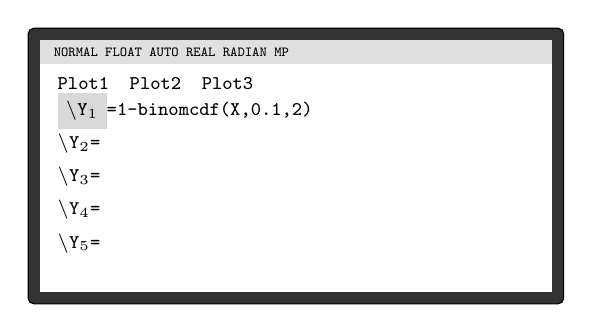
\begin{tikzpicture}[font=\ttfamily\scriptsize]\draw[rounded corners=2pt,fill=black!80] (-0.15,-3.05) rectangle (6.65,0.45);\fill[white] (0,-2.9) rectangle (6.5,0.3);\fill[black!12] (0,0) rectangle (6.5,0.3);\node[anchor=west,font=\ttfamily\tiny] at (0.05,0.15){NORMAL FLOAT AUTO REAL RADIAN MP};\node[anchor=west] at (0.1,-0.25){Plot1\ \ Plot2\ \ Plot3};\node[anchor=west] at (0.1,-0.6){\colorbox{black!15}{\textbackslash Y$_1$}=1-binomcdf(X,0.1,2)};\node[anchor=west] at (0.1,-1.02){\textbackslash Y$_2$=};\node[anchor=west] at (0.1,-1.44){\textbackslash Y$_3$=};\node[anchor=west] at (0.1,-1.86){\textbackslash Y$_4$=};\node[anchor=west] at (0.1,-2.28){\textbackslash Y$_5$=};\end{tikzpicture}\\[4pt]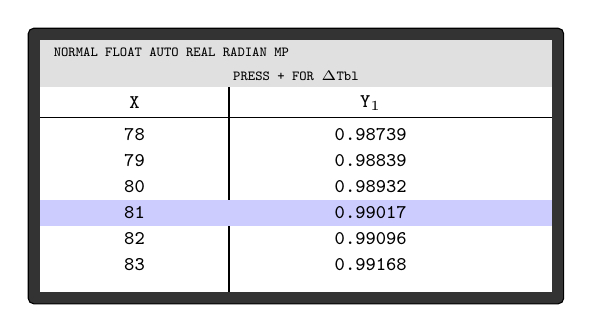
\begin{tikzpicture}[font=\ttfamily\scriptsize]\draw[rounded corners=2pt,fill=black!80] (-0.15,-3.05) rectangle (6.65,0.45);\fill[white] (0,-2.9) rectangle (6.5,0.3);\fill[black!12] (0,0) rectangle (6.5,0.3);\node[anchor=west,font=\ttfamily\tiny] at (0.05,0.15){NORMAL FLOAT AUTO REAL RADIAN MP};\fill[black!12] (0,-0.3) rectangle (6.5,0);\node[font=\ttfamily\tiny] at (3.25,-0.15){PRESS + FOR $\Delta$Tbl};\node at (1.2,-0.5){X};\node at (4.2,-0.5){Y$_1$};\draw (0,-0.68)--(6.5,-0.68);\draw (2.4,-0.3)--(2.4,-2.9);\node at (1.2,-0.90){78};\node at (4.2,-0.90){0.98739};\node at (1.2,-1.23){79};\node at (4.2,-1.23){0.98839};\node at (1.2,-1.56){80};\node at (4.2,-1.56){0.98932};\fill[blue!20] (0,-2.06) rectangle (6.5,-1.73);\node at (1.2,-1.89){81};\node at (4.2,-1.89){0.99017};\node at (1.2,-2.22){82};\node at (4.2,-2.22){0.99096};\node at (1.2,-2.55){83};\node at (4.2,-2.55){0.99168};\end{tikzpicture}\end{center}
\cdisp{\therefore\ n_{\min}&=81}
\end{minipage}\hfill
\begin{minipage}[t]{0.48\textwidth}
\exlab $X\sim\Bi{10}{p}$. Given that the mode of $X$ is $3$, find the range of $p$. {\color{gray}\footnotesize(At $p=\frac{3}{11}$ or $\frac{4}{11}$ there are two modes, so strict inequalities are used.)}
\cdisp{\Pp{X=3}&>\Pp{X=2}\\\nCr{10}{3}p^{3}(1-p)^{7}&>\nCr{10}{2}p^{2}(1-p)^{8}\\120p&>45(1-p)\\165p&>45\\p&>\dfrac{3}{11}\\\Pp{X=3}&>\Pp{X=4}\\\nCr{10}{3}p^{3}(1-p)^{7}&>\nCr{10}{4}p^{4}(1-p)^{6}\\120(1-p)&>210p\\120&>330p\\p&<\dfrac{4}{11}\\\therefore\ \dfrac{3}{11}&<p<\dfrac{4}{11}}
\end{minipage}
\par\medskip
\noindent\exlab The number of defective items in a box of $20$ is modelled by $X\sim\Bi{20}{0.3}$. A random sample of $50$ boxes is taken. By using a suitable approximation, estimate the probability that the mean number of defective items per box exceeds $6.2$.
\cdisp{\E(X)&=20(0.3)=6\\\Var(X)&=20(0.3)(0.7)=4.2}
$\because$ $N=50$ is large,
\[\bar{X}\sim\mathrm{N}\!\left(6,\dfrac{4.2}{50}\right)\text{ approximately by CLT}\]
\cdisp{\therefore\ \Pp{\bar{X}>6.2}&=0.245}
